\documentclass[twoside]{book}

% Packages required by doxygen
\usepackage{fixltx2e}
\usepackage{calc}
\usepackage{doxygen}
\usepackage[export]{adjustbox} % also loads graphicx
\usepackage{graphicx}
\usepackage[utf8]{inputenc}
\usepackage{makeidx}
\usepackage{multicol}
\usepackage{multirow}
\PassOptionsToPackage{warn}{textcomp}
\usepackage{textcomp}
\usepackage[nointegrals]{wasysym}
\usepackage[table]{xcolor}

% Font selection
\usepackage[T1]{fontenc}
\usepackage[scaled=.90]{helvet}
\usepackage{courier}
\usepackage{amssymb}
\usepackage{sectsty}
\renewcommand{\familydefault}{\sfdefault}
\allsectionsfont{%
  \fontseries{bc}\selectfont%
  \color{darkgray}%
}
\renewcommand{\DoxyLabelFont}{%
  \fontseries{bc}\selectfont%
  \color{darkgray}%
}
\newcommand{\+}{\discretionary{\mbox{\scriptsize$\hookleftarrow$}}{}{}}

% Page & text layout
\usepackage{geometry}
\geometry{%
  a4paper,%
  top=2.5cm,%
  bottom=2.5cm,%
  left=2.5cm,%
  right=2.5cm%
}
\tolerance=750
\hfuzz=15pt
\hbadness=750
\setlength{\emergencystretch}{15pt}
\setlength{\parindent}{0cm}
\setlength{\parskip}{3ex plus 2ex minus 2ex}
\makeatletter
\renewcommand{\paragraph}{%
  \@startsection{paragraph}{4}{0ex}{-1.0ex}{1.0ex}{%
    \normalfont\normalsize\bfseries\SS@parafont%
  }%
}
\renewcommand{\subparagraph}{%
  \@startsection{subparagraph}{5}{0ex}{-1.0ex}{1.0ex}{%
    \normalfont\normalsize\bfseries\SS@subparafont%
  }%
}
\makeatother

% Headers & footers
\usepackage{fancyhdr}
\pagestyle{fancyplain}
\fancyhead[LE]{\fancyplain{}{\bfseries\thepage}}
\fancyhead[CE]{\fancyplain{}{}}
\fancyhead[RE]{\fancyplain{}{\bfseries\leftmark}}
\fancyhead[LO]{\fancyplain{}{\bfseries\rightmark}}
\fancyhead[CO]{\fancyplain{}{}}
\fancyhead[RO]{\fancyplain{}{\bfseries\thepage}}
\fancyfoot[LE]{\fancyplain{}{}}
\fancyfoot[CE]{\fancyplain{}{}}
\fancyfoot[RE]{\fancyplain{}{\bfseries\scriptsize Generated by Doxygen }}
\fancyfoot[LO]{\fancyplain{}{\bfseries\scriptsize Generated by Doxygen }}
\fancyfoot[CO]{\fancyplain{}{}}
\fancyfoot[RO]{\fancyplain{}{}}
\renewcommand{\footrulewidth}{0.4pt}
\renewcommand{\chaptermark}[1]{%
  \markboth{#1}{}%
}
\renewcommand{\sectionmark}[1]{%
  \markright{\thesection\ #1}%
}

% Indices & bibliography
\usepackage{natbib}
\usepackage[titles]{tocloft}
\setcounter{tocdepth}{3}
\setcounter{secnumdepth}{5}
\makeindex

% Hyperlinks (required, but should be loaded last)
\usepackage{ifpdf}
\ifpdf
  \usepackage[pdftex,pagebackref=true]{hyperref}
\else
  \usepackage[ps2pdf,pagebackref=true]{hyperref}
\fi
\hypersetup{%
  colorlinks=true,%
  linkcolor=blue,%
  citecolor=blue,%
  unicode%
}

% Custom commands
\newcommand{\clearemptydoublepage}{%
  \newpage{\pagestyle{empty}\cleardoublepage}%
}

\usepackage{caption}
\captionsetup{labelsep=space,justification=centering,font={bf},singlelinecheck=off,skip=4pt,position=top}

%===== C O N T E N T S =====

\begin{document}

% Titlepage & ToC
\hypersetup{pageanchor=false,
             bookmarksnumbered=true,
             pdfencoding=unicode
            }
\pagenumbering{alph}
\begin{titlepage}
\vspace*{7cm}
\begin{center}%
{\Large Tri\+Cl \\[1ex]\large 0.\+1 }\\
\vspace*{1cm}
{\large Generated by Doxygen 1.8.13}\\
\end{center}
\end{titlepage}
\clearemptydoublepage
\pagenumbering{roman}
\tableofcontents
\clearemptydoublepage
\pagenumbering{arabic}
\hypersetup{pageanchor=true}

%--- Begin generated contents ---
\chapter{Data Structure Index}
\section{Data Structures}
Here are the data structures with brief descriptions\+:\begin{DoxyCompactList}
\item\contentsline{section}{\hyperlink{structtricl_1_1angle}{tricl\+::angle} }{\pageref{structtricl_1_1angle}}{}
\item\contentsline{section}{\hyperlink{structtricl_1_1angle__type}{tricl\+::angle\+\_\+type} }{\pageref{structtricl_1_1angle__type}}{}
\item\contentsline{section}{\hyperlink{structtricl_1_1entity__type__pair}{tricl\+::entity\+\_\+type\+\_\+pair} }{\pageref{structtricl_1_1entity__type__pair}}{}
\item\contentsline{section}{\hyperlink{structtricl_1_1event}{tricl\+::event} }{\pageref{structtricl_1_1event}}{}
\item\contentsline{section}{\hyperlink{structtricl_1_1event__data}{tricl\+::event\+\_\+data} }{\pageref{structtricl_1_1event__data}}{}
\item\contentsline{section}{\hyperlink{structtricl_1_1event__type}{tricl\+::event\+\_\+type} }{\pageref{structtricl_1_1event__type}}{}
\item\contentsline{section}{\hyperlink{structstd_1_1hash_3_01angle_01_4}{std\+::hash$<$ angle $>$} }{\pageref{structstd_1_1hash_3_01angle_01_4}}{}
\item\contentsline{section}{\hyperlink{structstd_1_1hash_3_01angle__type_01_4}{std\+::hash$<$ angle\+\_\+type $>$} }{\pageref{structstd_1_1hash_3_01angle__type_01_4}}{}
\item\contentsline{section}{\hyperlink{structstd_1_1hash_3_01entity__type__pair_01_4}{std\+::hash$<$ entity\+\_\+type\+\_\+pair $>$} }{\pageref{structstd_1_1hash_3_01entity__type__pair_01_4}}{}
\item\contentsline{section}{\hyperlink{structstd_1_1hash_3_01event_01_4}{std\+::hash$<$ event $>$} }{\pageref{structstd_1_1hash_3_01event_01_4}}{}
\item\contentsline{section}{\hyperlink{structstd_1_1hash_3_01event__type_01_4}{std\+::hash$<$ event\+\_\+type $>$} }{\pageref{structstd_1_1hash_3_01event__type_01_4}}{}
\item\contentsline{section}{\hyperlink{structstd_1_1hash_3_01influence__type_01_4}{std\+::hash$<$ influence\+\_\+type $>$} }{\pageref{structstd_1_1hash_3_01influence__type_01_4}}{}
\item\contentsline{section}{\hyperlink{structstd_1_1hash_3_01inleg_01_4}{std\+::hash$<$ inleg $>$} }{\pageref{structstd_1_1hash_3_01inleg_01_4}}{}
\item\contentsline{section}{\hyperlink{structstd_1_1hash_3_01link_01_4}{std\+::hash$<$ link $>$} }{\pageref{structstd_1_1hash_3_01link_01_4}}{}
\item\contentsline{section}{\hyperlink{structstd_1_1hash_3_01link__type_01_4}{std\+::hash$<$ link\+\_\+type $>$} }{\pageref{structstd_1_1hash_3_01link__type_01_4}}{}
\item\contentsline{section}{\hyperlink{structstd_1_1hash_3_01outleg_01_4}{std\+::hash$<$ outleg $>$} }{\pageref{structstd_1_1hash_3_01outleg_01_4}}{}
\item\contentsline{section}{\hyperlink{structtricl_1_1influence__type}{tricl\+::influence\+\_\+type} }{\pageref{structtricl_1_1influence__type}}{}
\item\contentsline{section}{\hyperlink{structtricl_1_1inleg}{tricl\+::inleg} }{\pageref{structtricl_1_1inleg}}{}
\item\contentsline{section}{\hyperlink{structtricl_1_1link}{tricl\+::link} }{\pageref{structtricl_1_1link}}{}
\item\contentsline{section}{\hyperlink{structtricl_1_1link__type}{tricl\+::link\+\_\+type} }{\pageref{structtricl_1_1link__type}}{}
\item\contentsline{section}{\hyperlink{structtricl_1_1outleg}{tricl\+::outleg} }{\pageref{structtricl_1_1outleg}}{}
\end{DoxyCompactList}

\chapter{Data Structure Documentation}
\hypertarget{structangle}{}\section{angle Struct Reference}
\label{structangle}\index{angle@{angle}}
\subsection*{Data Fields}
\begin{DoxyCompactItemize}
\item 
\mbox{\Hypertarget{structangle_ae2506f4585814e8db2472cc9665bc230}\label{structangle_ae2506f4585814e8db2472cc9665bc230}} 
relationship\+\_\+or\+\_\+action\+\_\+type {\bfseries rat12}
\item 
\mbox{\Hypertarget{structangle_a8be7ceadded85927d37e07a37f73e126}\label{structangle_a8be7ceadded85927d37e07a37f73e126}} 
entity {\bfseries e2}
\item 
\mbox{\Hypertarget{structangle_a718f64e8c5e13b0d0a3be99a034b87fe}\label{structangle_a718f64e8c5e13b0d0a3be99a034b87fe}} 
relationship\+\_\+or\+\_\+action\+\_\+type {\bfseries rat23}
\end{DoxyCompactItemize}
\subsection*{Friends}
\begin{DoxyCompactItemize}
\item 
\mbox{\Hypertarget{structangle_a08af3ce953cf2a9246fc60278c929a52}\label{structangle_a08af3ce953cf2a9246fc60278c929a52}} 
bool {\bfseries operator==} (const \hyperlink{structangle}{angle} \&left, const \hyperlink{structangle}{angle} \&right)
\end{DoxyCompactItemize}


The documentation for this struct was generated from the following file\+:\begin{DoxyCompactItemize}
\item 
src/\hyperlink{data__model_8h}{data\+\_\+model.\+h}\end{DoxyCompactItemize}

\hypertarget{structangle__type}{}\section{angle\+\_\+type Struct Reference}
\label{structangle__type}\index{angle\+\_\+type@{angle\+\_\+type}}
\subsection*{Data Fields}
\begin{DoxyCompactItemize}
\item 
\mbox{\Hypertarget{structangle__type_a748f65a3ae97f3dba1cac69d40330f42}\label{structangle__type_a748f65a3ae97f3dba1cac69d40330f42}} 
const relationship\+\_\+or\+\_\+action\+\_\+type {\bfseries rat12}
\item 
\mbox{\Hypertarget{structangle__type_a597582b9649e36a41e8f0a5e0ea50c66}\label{structangle__type_a597582b9649e36a41e8f0a5e0ea50c66}} 
const entity\+\_\+type {\bfseries et2}
\item 
\mbox{\Hypertarget{structangle__type_ad98ed08839b6c50759ae01fb72338cb9}\label{structangle__type_ad98ed08839b6c50759ae01fb72338cb9}} 
const relationship\+\_\+or\+\_\+action\+\_\+type {\bfseries rat23}
\end{DoxyCompactItemize}
\subsection*{Friends}
\begin{DoxyCompactItemize}
\item 
\mbox{\Hypertarget{structangle__type_a259cbf4e32421b1e65066025fa86e999}\label{structangle__type_a259cbf4e32421b1e65066025fa86e999}} 
bool {\bfseries operator==} (const \hyperlink{structangle__type}{angle\+\_\+type} \&left, const \hyperlink{structangle__type}{angle\+\_\+type} \&right)
\end{DoxyCompactItemize}


The documentation for this struct was generated from the following file\+:\begin{DoxyCompactItemize}
\item 
src/data\+\_\+model.\+h\end{DoxyCompactItemize}

\hypertarget{structentity__type__pair}{}\section{entity\+\_\+type\+\_\+pair Struct Reference}
\label{structentity__type__pair}\index{entity\+\_\+type\+\_\+pair@{entity\+\_\+type\+\_\+pair}}
\subsection*{Data Fields}
\begin{DoxyCompactItemize}
\item 
\mbox{\Hypertarget{structentity__type__pair_aac00f0d65f32a57745f708c2b1cd9b1f}\label{structentity__type__pair_aac00f0d65f32a57745f708c2b1cd9b1f}} 
const entity\+\_\+type {\bfseries et1}
\item 
\mbox{\Hypertarget{structentity__type__pair_af1298e0bc96d48d5ae9b6bcdd0430ea3}\label{structentity__type__pair_af1298e0bc96d48d5ae9b6bcdd0430ea3}} 
const entity\+\_\+type {\bfseries et3}
\end{DoxyCompactItemize}
\subsection*{Friends}
\begin{DoxyCompactItemize}
\item 
\mbox{\Hypertarget{structentity__type__pair_ab148ef41047fcbd537a8f98b11e11045}\label{structentity__type__pair_ab148ef41047fcbd537a8f98b11e11045}} 
bool {\bfseries operator==} (const \hyperlink{structentity__type__pair}{entity\+\_\+type\+\_\+pair} \&left, const \hyperlink{structentity__type__pair}{entity\+\_\+type\+\_\+pair} \&right)
\end{DoxyCompactItemize}


The documentation for this struct was generated from the following file\+:\begin{DoxyCompactItemize}
\item 
src/\hyperlink{data__model_8h}{data\+\_\+model.\+h}\end{DoxyCompactItemize}

\hypertarget{structevent}{}\section{event Struct Reference}
\label{structevent}\index{event@{event}}
\subsection*{Data Fields}
\begin{DoxyCompactItemize}
\item 
\mbox{\Hypertarget{structevent_ac32b92ff80a203fd7c27e7313e4429d2}\label{structevent_ac32b92ff80a203fd7c27e7313e4429d2}} 
event\+\_\+class {\bfseries ec}
\item 
\mbox{\Hypertarget{structevent_a829a8f5791c5189324ffa115608f20ee}\label{structevent_a829a8f5791c5189324ffa115608f20ee}} 
entity {\bfseries e1}
\item 
\mbox{\Hypertarget{structevent_a4bf1c0667655028954126c33657330c9}\label{structevent_a4bf1c0667655028954126c33657330c9}} 
relationship\+\_\+or\+\_\+action\+\_\+type {\bfseries rat13}
\item 
\mbox{\Hypertarget{structevent_ac7c3b30ab1c81bece0be283c615a7015}\label{structevent_ac7c3b30ab1c81bece0be283c615a7015}} 
entity {\bfseries e3}
\end{DoxyCompactItemize}
\subsection*{Friends}
\begin{DoxyCompactItemize}
\item 
\mbox{\Hypertarget{structevent_a3dd0c9c41d63a2d2171cffc7dfa14d6c}\label{structevent_a3dd0c9c41d63a2d2171cffc7dfa14d6c}} 
bool {\bfseries operator==} (const \hyperlink{structevent}{event} \&left, const \hyperlink{structevent}{event} \&right)
\item 
\mbox{\Hypertarget{structevent_a4d697ad127dbb87399c435f1e216ec8a}\label{structevent_a4d697ad127dbb87399c435f1e216ec8a}} 
ostream \& {\bfseries operator$<$$<$} (ostream \&os, const \hyperlink{structevent}{event} \&ev)
\end{DoxyCompactItemize}


The documentation for this struct was generated from the following file\+:\begin{DoxyCompactItemize}
\item 
src/data\+\_\+model.\+h\end{DoxyCompactItemize}

\hypertarget{structevent__data}{}\section{event\+\_\+data Struct Reference}
\label{structevent__data}\index{event\+\_\+data@{event\+\_\+data}}
\subsection*{Data Fields}
\begin{DoxyCompactItemize}
\item 
int {\bfseries n\+\_\+angles} = 0\hypertarget{structevent__data_a4ac8163657589d149ed034f321b61ce9}{}\label{structevent__data_a4ac8163657589d149ed034f321b61ce9}

\item 
rate {\bfseries attempt\+\_\+rate}\hypertarget{structevent__data_aa12da1e46a4e8e401433e90fd97fc015}{}\label{structevent__data_aa12da1e46a4e8e401433e90fd97fc015}

\item 
probunit {\bfseries success\+\_\+probunits}\hypertarget{structevent__data_a74dff9b3b11ccf5cc10e96a54c582f0f}{}\label{structevent__data_a74dff9b3b11ccf5cc10e96a54c582f0f}

\item 
timepoint {\bfseries t} = -\/I\+N\+F\+I\+N\+I\+TY\hypertarget{structevent__data_aa2f4362fb8d987420d6941e29cb50710}{}\label{structevent__data_aa2f4362fb8d987420d6941e29cb50710}

\end{DoxyCompactItemize}
\subsection*{Friends}
\begin{DoxyCompactItemize}
\item 
ostream \& {\bfseries operator$<$$<$} (ostream \&os, const \hyperlink{structevent__data}{event\+\_\+data} \&evd)\hypertarget{structevent__data_a39ddcc1bb1a2d01e9868f33afdb1beba}{}\label{structevent__data_a39ddcc1bb1a2d01e9868f33afdb1beba}

\end{DoxyCompactItemize}


The documentation for this struct was generated from the following file\+:\begin{DoxyCompactItemize}
\item 
src/\hyperlink{data__model_8h}{data\+\_\+model.\+h}\end{DoxyCompactItemize}

\hypertarget{structevent__type}{}\section{event\+\_\+type Struct Reference}
\label{structevent__type}\index{event\+\_\+type@{event\+\_\+type}}
\subsection*{Data Fields}
\begin{DoxyCompactItemize}
\item 
\mbox{\Hypertarget{structevent__type_a56c49b8b98c18fb39797a92285387eca}\label{structevent__type_a56c49b8b98c18fb39797a92285387eca}} 
const event\+\_\+class {\bfseries ec}
\item 
\mbox{\Hypertarget{structevent__type_a127abbfe7df2d4e442ef38c4d12b6dd2}\label{structevent__type_a127abbfe7df2d4e442ef38c4d12b6dd2}} 
const entity\+\_\+type {\bfseries et1}
\item 
\mbox{\Hypertarget{structevent__type_a7fe60f7b335a887a54c37c4b9fcfb400}\label{structevent__type_a7fe60f7b335a887a54c37c4b9fcfb400}} 
const relationship\+\_\+or\+\_\+action\+\_\+type {\bfseries rat13}
\item 
\mbox{\Hypertarget{structevent__type_a685ac2668f6698357089949c495f6fe3}\label{structevent__type_a685ac2668f6698357089949c495f6fe3}} 
const entity\+\_\+type {\bfseries et3}
\end{DoxyCompactItemize}
\subsection*{Friends}
\begin{DoxyCompactItemize}
\item 
\mbox{\Hypertarget{structevent__type_ac6ea5340a97cf343356e390f082881de}\label{structevent__type_ac6ea5340a97cf343356e390f082881de}} 
bool {\bfseries operator==} (const \hyperlink{structevent__type}{event\+\_\+type} \&left, const \hyperlink{structevent__type}{event\+\_\+type} \&right)
\item 
\mbox{\Hypertarget{structevent__type_aaeec0fa308de88d46a6abc86499fe596}\label{structevent__type_aaeec0fa308de88d46a6abc86499fe596}} 
ostream \& {\bfseries operator$<$$<$} (ostream \&os, const \hyperlink{structevent__type}{event\+\_\+type} \&e)
\end{DoxyCompactItemize}


The documentation for this struct was generated from the following file\+:\begin{DoxyCompactItemize}
\item 
src/data\+\_\+model.\+h\end{DoxyCompactItemize}

\hypertarget{structstd_1_1hash_3_01angle_01_4}{}\section{std\+:\+:hash$<$ angle $>$ Struct Template Reference}
\label{structstd_1_1hash_3_01angle_01_4}\index{std\+::hash$<$ angle $>$@{std\+::hash$<$ angle $>$}}
\subsection*{Public Member Functions}
\begin{DoxyCompactItemize}
\item 
\mbox{\Hypertarget{structstd_1_1hash_3_01angle_01_4_a545cf76d8119d6f602bbf0d28804bd87}\label{structstd_1_1hash_3_01angle_01_4_a545cf76d8119d6f602bbf0d28804bd87}} 
size\+\_\+t {\bfseries operator()} (const \hyperlink{structangle}{angle} \&a) const
\end{DoxyCompactItemize}


The documentation for this struct was generated from the following file\+:\begin{DoxyCompactItemize}
\item 
src/data\+\_\+model.\+h\end{DoxyCompactItemize}

\hypertarget{structstd_1_1hash_3_01angle__type_01_4}{}\section{std\+:\+:hash$<$ angle\+\_\+type $>$ Struct Template Reference}
\label{structstd_1_1hash_3_01angle__type_01_4}\index{std\+::hash$<$ angle\+\_\+type $>$@{std\+::hash$<$ angle\+\_\+type $>$}}
\subsection*{Public Member Functions}
\begin{DoxyCompactItemize}
\item 
\mbox{\Hypertarget{structstd_1_1hash_3_01angle__type_01_4_a7057058e8815eaaee739fe49d1e76d58}\label{structstd_1_1hash_3_01angle__type_01_4_a7057058e8815eaaee739fe49d1e76d58}} 
size\+\_\+t {\bfseries operator()} (const \hyperlink{structtricl_1_1angle__type}{angle\+\_\+type} \&at) const
\end{DoxyCompactItemize}


The documentation for this struct was generated from the following file\+:\begin{DoxyCompactItemize}
\item 
src/\hyperlink{data__model_8h}{data\+\_\+model.\+h}\end{DoxyCompactItemize}

\hypertarget{structstd_1_1hash_3_01entity__type__pair_01_4}{}\section{std\+:\+:hash$<$ entity\+\_\+type\+\_\+pair $>$ Struct Template Reference}
\label{structstd_1_1hash_3_01entity__type__pair_01_4}\index{std\+::hash$<$ entity\+\_\+type\+\_\+pair $>$@{std\+::hash$<$ entity\+\_\+type\+\_\+pair $>$}}
\subsection*{Public Member Functions}
\begin{DoxyCompactItemize}
\item 
size\+\_\+t {\bfseries operator()} (const \hyperlink{structentity__type__pair}{entity\+\_\+type\+\_\+pair} \&etp) const \hypertarget{structstd_1_1hash_3_01entity__type__pair_01_4_a5455d0509fcec02e7ba7769af2c912f7}{}\label{structstd_1_1hash_3_01entity__type__pair_01_4_a5455d0509fcec02e7ba7769af2c912f7}

\end{DoxyCompactItemize}


The documentation for this struct was generated from the following file\+:\begin{DoxyCompactItemize}
\item 
src/\hyperlink{data__model_8h}{data\+\_\+model.\+h}\end{DoxyCompactItemize}

\hypertarget{structstd_1_1hash_3_01event_01_4}{}\section{std\+:\+:hash$<$ event $>$ Struct Template Reference}
\label{structstd_1_1hash_3_01event_01_4}\index{std\+::hash$<$ event $>$@{std\+::hash$<$ event $>$}}
\subsection*{Public Member Functions}
\begin{DoxyCompactItemize}
\item 
size\+\_\+t {\bfseries operator()} (const \hyperlink{structevent}{event} \&ev) const \hypertarget{structstd_1_1hash_3_01event_01_4_a316907f66e6012bbde95cd972a650f42}{}\label{structstd_1_1hash_3_01event_01_4_a316907f66e6012bbde95cd972a650f42}

\end{DoxyCompactItemize}


The documentation for this struct was generated from the following file\+:\begin{DoxyCompactItemize}
\item 
src/\hyperlink{data__model_8h}{data\+\_\+model.\+h}\end{DoxyCompactItemize}

\hypertarget{structstd_1_1hash_3_01event__type_01_4}{}\section{std\+:\+:hash$<$ event\+\_\+type $>$ Struct Template Reference}
\label{structstd_1_1hash_3_01event__type_01_4}\index{std\+::hash$<$ event\+\_\+type $>$@{std\+::hash$<$ event\+\_\+type $>$}}
\subsection*{Public Member Functions}
\begin{DoxyCompactItemize}
\item 
\mbox{\Hypertarget{structstd_1_1hash_3_01event__type_01_4_ad45f8465347bc54724583f2abb7c7e8f}\label{structstd_1_1hash_3_01event__type_01_4_ad45f8465347bc54724583f2abb7c7e8f}} 
size\+\_\+t {\bfseries operator()} (const \hyperlink{structevent__type}{event\+\_\+type} \&evt) const
\end{DoxyCompactItemize}


The documentation for this struct was generated from the following file\+:\begin{DoxyCompactItemize}
\item 
src/\hyperlink{data__model_8h}{data\+\_\+model.\+h}\end{DoxyCompactItemize}

\hypertarget{structstd_1_1hash_3_01influence__type_01_4}{}\section{std\+:\+:hash$<$ influence\+\_\+type $>$ Struct Template Reference}
\label{structstd_1_1hash_3_01influence__type_01_4}\index{std\+::hash$<$ influence\+\_\+type $>$@{std\+::hash$<$ influence\+\_\+type $>$}}
\subsection*{Public Member Functions}
\begin{DoxyCompactItemize}
\item 
size\+\_\+t {\bfseries operator()} (const \hyperlink{structinfluence__type}{influence\+\_\+type} \&inflt) const \hypertarget{structstd_1_1hash_3_01influence__type_01_4_ae8d3b8ef874ef449b3ff3df4df18324e}{}\label{structstd_1_1hash_3_01influence__type_01_4_ae8d3b8ef874ef449b3ff3df4df18324e}

\end{DoxyCompactItemize}


The documentation for this struct was generated from the following file\+:\begin{DoxyCompactItemize}
\item 
src/\hyperlink{data__model_8h}{data\+\_\+model.\+h}\end{DoxyCompactItemize}

\hypertarget{structstd_1_1hash_3_01leg_01_4}{}\section{std\+:\+:hash$<$ leg $>$ Struct Template Reference}
\label{structstd_1_1hash_3_01leg_01_4}\index{std\+::hash$<$ leg $>$@{std\+::hash$<$ leg $>$}}
\subsection*{Public Member Functions}
\begin{DoxyCompactItemize}
\item 
\mbox{\Hypertarget{structstd_1_1hash_3_01leg_01_4_ae0aff468b8cdeac8d5a1fab1eed668c8}\label{structstd_1_1hash_3_01leg_01_4_ae0aff468b8cdeac8d5a1fab1eed668c8}} 
size\+\_\+t {\bfseries operator()} (const \hyperlink{structleg}{leg} \&l) const
\end{DoxyCompactItemize}


The documentation for this struct was generated from the following file\+:\begin{DoxyCompactItemize}
\item 
src/\hyperlink{data__model_8h}{data\+\_\+model.\+h}\end{DoxyCompactItemize}

\hypertarget{structstd_1_1hash_3_01link_01_4}{}\section{std\+:\+:hash$<$ link $>$ Struct Template Reference}
\label{structstd_1_1hash_3_01link_01_4}\index{std\+::hash$<$ link $>$@{std\+::hash$<$ link $>$}}
\subsection*{Public Member Functions}
\begin{DoxyCompactItemize}
\item 
size\+\_\+t {\bfseries operator()} (const \hyperlink{structlink}{link} \&l) const \hypertarget{structstd_1_1hash_3_01link_01_4_a7f52e43158cdd69f97bb2601b93c3c04}{}\label{structstd_1_1hash_3_01link_01_4_a7f52e43158cdd69f97bb2601b93c3c04}

\end{DoxyCompactItemize}


The documentation for this struct was generated from the following file\+:\begin{DoxyCompactItemize}
\item 
src/\hyperlink{data__model_8h}{data\+\_\+model.\+h}\end{DoxyCompactItemize}

\hypertarget{structstd_1_1hash_3_01link__type_01_4}{}\section{std\+:\+:hash$<$ link\+\_\+type $>$ Struct Template Reference}
\label{structstd_1_1hash_3_01link__type_01_4}\index{std\+::hash$<$ link\+\_\+type $>$@{std\+::hash$<$ link\+\_\+type $>$}}
\subsection*{Public Member Functions}
\begin{DoxyCompactItemize}
\item 
size\+\_\+t {\bfseries operator()} (const \hyperlink{structlink__type}{link\+\_\+type} \&lt) const \hypertarget{structstd_1_1hash_3_01link__type_01_4_a61dd62f400ac5e129f161447b008117a}{}\label{structstd_1_1hash_3_01link__type_01_4_a61dd62f400ac5e129f161447b008117a}

\end{DoxyCompactItemize}


The documentation for this struct was generated from the following file\+:\begin{DoxyCompactItemize}
\item 
src/\hyperlink{data__model_8h}{data\+\_\+model.\+h}\end{DoxyCompactItemize}

\hypertarget{structinfluence__type}{}\section{influence\+\_\+type Struct Reference}
\label{structinfluence__type}\index{influence\+\_\+type@{influence\+\_\+type}}


Collaboration diagram for influence\+\_\+type\+:\nopagebreak
\begin{figure}[H]
\begin{center}
\leavevmode
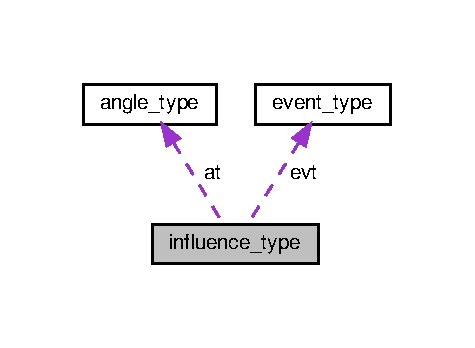
\includegraphics[width=228pt]{df/d32/structinfluence__type__coll__graph}
\end{center}
\end{figure}
\subsection*{Data Fields}
\begin{DoxyCompactItemize}
\item 
\mbox{\Hypertarget{structinfluence__type_a54609d8fd03b51d5a1961db4739af731}\label{structinfluence__type_a54609d8fd03b51d5a1961db4739af731}} 
const \hyperlink{structevent__type}{event\+\_\+type} {\bfseries evt}
\item 
\mbox{\Hypertarget{structinfluence__type_a1232197d61a8bebc4d5c64ec54745aa3}\label{structinfluence__type_a1232197d61a8bebc4d5c64ec54745aa3}} 
const \hyperlink{structangle__type}{angle\+\_\+type} {\bfseries at}
\end{DoxyCompactItemize}
\subsection*{Friends}
\begin{DoxyCompactItemize}
\item 
\mbox{\Hypertarget{structinfluence__type_a4f5b42686b09f580c15f8fa9f3aa296f}\label{structinfluence__type_a4f5b42686b09f580c15f8fa9f3aa296f}} 
bool {\bfseries operator==} (const \hyperlink{structinfluence__type}{influence\+\_\+type} \&left, const \hyperlink{structinfluence__type}{influence\+\_\+type} \&right)
\end{DoxyCompactItemize}


The documentation for this struct was generated from the following file\+:\begin{DoxyCompactItemize}
\item 
src/\hyperlink{data__model_8h}{data\+\_\+model.\+h}\end{DoxyCompactItemize}

\hypertarget{structleg}{}\section{leg Struct Reference}
\label{structleg}\index{leg@{leg}}
\subsection*{Data Fields}
\begin{DoxyCompactItemize}
\item 
\mbox{\Hypertarget{structleg_a25bc8afc8fdc636963b7cae1f5bbaa3b}\label{structleg_a25bc8afc8fdc636963b7cae1f5bbaa3b}} 
const entity {\bfseries e}
\item 
\mbox{\Hypertarget{structleg_a8136189afab60f788096b94d01b91d1c}\label{structleg_a8136189afab60f788096b94d01b91d1c}} 
const relationship\+\_\+or\+\_\+action\+\_\+type {\bfseries r}
\end{DoxyCompactItemize}
\subsection*{Friends}
\begin{DoxyCompactItemize}
\item 
\mbox{\Hypertarget{structleg_a79d778afcc9e6d9a84a5e5621d9e7223}\label{structleg_a79d778afcc9e6d9a84a5e5621d9e7223}} 
bool {\bfseries operator==} (const \hyperlink{structleg}{leg} \&left, const \hyperlink{structleg}{leg} \&right)
\item 
\mbox{\Hypertarget{structleg_a050cb42dbf3c9c1063f14234d5902bee}\label{structleg_a050cb42dbf3c9c1063f14234d5902bee}} 
bool {\bfseries operator$<$} (const \hyperlink{structleg}{leg} \&left, const \hyperlink{structleg}{leg} \&right)
\end{DoxyCompactItemize}


The documentation for this struct was generated from the following file\+:\begin{DoxyCompactItemize}
\item 
src/\hyperlink{data__model_8h}{data\+\_\+model.\+h}\end{DoxyCompactItemize}

\hypertarget{structlink}{}\section{link Struct Reference}
\label{structlink}\index{link@{link}}
\subsection*{Data Fields}
\begin{DoxyCompactItemize}
\item 
\mbox{\Hypertarget{structlink_a5a3eda51498d357ce568579c1518ddc0}\label{structlink_a5a3eda51498d357ce568579c1518ddc0}} 
const entity {\bfseries e1}
\item 
\mbox{\Hypertarget{structlink_a926504798d48f1e25b0c5217ef96bd9a}\label{structlink_a926504798d48f1e25b0c5217ef96bd9a}} 
const relationship\+\_\+or\+\_\+action\+\_\+type {\bfseries rat13}
\item 
\mbox{\Hypertarget{structlink_ab87c26d64d781c9173d767772a45e9f0}\label{structlink_ab87c26d64d781c9173d767772a45e9f0}} 
const entity {\bfseries e3}
\end{DoxyCompactItemize}
\subsection*{Friends}
\begin{DoxyCompactItemize}
\item 
\mbox{\Hypertarget{structlink_a383e61e15072ef3fe9e16102dea483e0}\label{structlink_a383e61e15072ef3fe9e16102dea483e0}} 
bool {\bfseries operator==} (const \hyperlink{structlink}{link} \&left, const \hyperlink{structlink}{link} \&right)
\item 
\mbox{\Hypertarget{structlink_af79bc13140c8180154526642748b0c33}\label{structlink_af79bc13140c8180154526642748b0c33}} 
bool {\bfseries operator$<$} (const \hyperlink{structlink}{link} \&left, const \hyperlink{structlink}{link} \&right)
\end{DoxyCompactItemize}


The documentation for this struct was generated from the following file\+:\begin{DoxyCompactItemize}
\item 
src/\hyperlink{data__model_8h}{data\+\_\+model.\+h}\end{DoxyCompactItemize}

\hypertarget{structlink__type}{}\section{link\+\_\+type Struct Reference}
\label{structlink__type}\index{link\+\_\+type@{link\+\_\+type}}
\subsection*{Data Fields}
\begin{DoxyCompactItemize}
\item 
\mbox{\Hypertarget{structlink__type_aa1e1406306efb10b6c71e6425df2405d}\label{structlink__type_aa1e1406306efb10b6c71e6425df2405d}} 
const entity\+\_\+type {\bfseries et1}
\item 
\mbox{\Hypertarget{structlink__type_ac178aea7e3b72e3579ea365625291c4a}\label{structlink__type_ac178aea7e3b72e3579ea365625291c4a}} 
const relationship\+\_\+or\+\_\+action\+\_\+type {\bfseries rat13}
\item 
\mbox{\Hypertarget{structlink__type_a5d2db20b11fedaab93e193fce2e205a8}\label{structlink__type_a5d2db20b11fedaab93e193fce2e205a8}} 
const entity\+\_\+type {\bfseries et3}
\end{DoxyCompactItemize}
\subsection*{Friends}
\begin{DoxyCompactItemize}
\item 
\mbox{\Hypertarget{structlink__type_ae75460e218908d70af1163248317096e}\label{structlink__type_ae75460e218908d70af1163248317096e}} 
bool {\bfseries operator==} (const \hyperlink{structlink__type}{link\+\_\+type} \&left, const \hyperlink{structlink__type}{link\+\_\+type} \&right)
\item 
\mbox{\Hypertarget{structlink__type_a3b1d9aca31b4d38961fafd8f10732bea}\label{structlink__type_a3b1d9aca31b4d38961fafd8f10732bea}} 
ostream \& {\bfseries operator$<$$<$} (ostream \&os, const \hyperlink{structlink__type}{link\+\_\+type} \&lt)
\end{DoxyCompactItemize}


The documentation for this struct was generated from the following file\+:\begin{DoxyCompactItemize}
\item 
src/\hyperlink{data__model_8h}{data\+\_\+model.\+h}\end{DoxyCompactItemize}

%--- End generated contents ---

% Index
\backmatter
\newpage
\phantomsection
\clearemptydoublepage
\addcontentsline{toc}{chapter}{Index}
\printindex

\end{document}
